%! Author = CaptSiro
%! Date = 11/26/2025

% Preamble
\documentclass{ctu/class/ctuthesis}

% Packages
\usepackage{amsmath}
%\usepackage[colorlinks=true, allcolors=blue]{hyperref}
\usepackage{float}
\usepackage[backend=biber,style=numeric]{biblatex}
\usepackage{pgf}
\usepackage{url}
\usepackage{tikz}
\usepackage{csquotes}
\usepackage{listings}
\usetikzlibrary{arrows.meta, positioning}
\addbibresource{references.bib}

\ctusetup{
    xdoctype = B,
    xfaculty = F3,
    mainlanguage = english,
    titlelanguage = english,
    doctype-english = {Bachelor Thesis},
    doctype-czech = {Bakalářská práce},
    title-english = {Design and Implementation of a PHP Web Application Framework with AI Support for Website Generation and Management},
    title-czech = {Návrh a implementace webového aplikačního frameworku v PHP s podporou umělé inteligence pro generování a správu webových stránek},
    keywords-english = {content management system, PHP web framework, generative artificial intelligence, natural language processing},
    keywords-czech = {systém pro správu obsahu, webový PHP framework, generativní umělá inteligence, zpracování přirozeného jazyka},
    department-english = {Department of Computer Graphics and Interaction},
    author = {Jan Horák},
    supervisor = {Mgr. Egor Ulianov},
    supervisor-address = {Department of Computer Graphics and Interaction FEE},
    fieldofstudy-english = {Open Informatics},
    subfieldofstudy-english = {Computer Games and Graphics},
    fieldofstudy-czech = {Otevřená informatika},
    subfieldofstudy-czech = {Počítačové hry a grafika},
    month = 5,
    year = 2026,
}

\ctuprocess

\begin{abstract-english}
    This thesis presents the design and implementation of a prototype full-stack framework written in PHP\@.
    The framework enables transforming requests in natural language into deployable website.
    The Generative AI acts as assistive layer that supports website structure creation from suggestion,
    generating content, composing UI blocks, and preparing templates or configuration.
    The AI layer allows human control over all generated outputs.

    The framework provides core full-stack web application functionality, including routing, controllers, middleware,
    templating, validation, persistence, authentication.
    Using the core functionalities, CMS features are implemented, which include website management, content,
    media, and publishing management with draft and published states.
    Role-based access control model is present in the framework and supports anonymous users, editors, and administrators.
    The frameworks supports multi-page applications using predefined page templates, including home page,
    a generic content page, an article list, an article detail, and a contact page.

    The AI-Generation implemented in the prototype must cover website structure generation, UI blocks generation,
    and proposing modifications of an existing page based on a natural-language request.
    The framework is validated through the creation of three websites, for which the full workflow from initial request
    to publication is documented.
    The evaluation includes CMS functionality of the system, AI-Generation, and basic metrics such as requirement coverage,
    number of manual interventions, and time to publishable state.
    This thesis concludes with an overview of results and identified limitations.
\end{abstract-english}
\begin{abstract-czech}
    Tato bakalářská práce představuje návrh a implementaci prototypu full-stack frameworku napsaného v jazyce PHP\@.
    Tento framework umožňuje převádět požadavky v přirozeném jazyce na funkční webové stránky.
    Generativní AI funguje jako pomocná vrstva, která podporuje návrh struktury webových stránek,
    generování obsahu, sestavování bloků uživatelského rozhraní a přípravu šablon či konfigurace.
    AI vrstva umožňuje uživateli kontrolovat všechny generované výstupy.

    Tento framework poskytuje základní funkce pro full-stack webové aplikace, včetně směrování, controllerů, middlewaru,
    vykreslování šablon, validace, ukládání dat a autentizace.
    Pomocí těchto základních funkcí jsou implementovány CMS funkce, které zahrnují správu webových stránek, obsahu,
    médií a publikování se stavy konceptu a publikovaného obsahu.
    Framework obsahuje model pro řízení přístupu založený na rolích a podporuje anonymní uživatele, editory a administrátory.
    Framework podporuje vícestránkové aplikace využívající předdefinované šablony stránek, včetně domovské stránky,
    obecné stránky s obsahem, seznamu článků, detailu článku a kontaktní stránky.

    Funkce generování pomocí AI implementovaná v prototypu musí zahrnovat generování struktury webových stránek, generování bloků uživatelského rozhraní
    a navrhování úprav stávající stránky na základě požadavku v přirozeném jazyce.
    Framework je ověřen vytvořením tří webových stránek, u nichž je zdokumentován celý pracovní postup od počátečního požadavku
    až po zveřejnění.
    Hodnocení zahrnuje funkčnost systému CMS, generování pomocí AI a základní metriky, jako je pokrytí požadavků,
    počet ručních úprav a doba do dosažení stavu vhodného ke zveřejnění.
    Tato práce končí přehledem výsledků a identifikovaných omezení.
\end{abstract-czech}

\begin{thanks}
    I would like to express my gratitude to my mother for her continuous support, patience,
    and encouragement throughout my studies and during the preparation of this thesis.

    I also thank my family for their support and understanding, which helped me stay motivated during my studies.

    Finally, I would like to thank my friends for their encouragement, helpful discussions,
    and for making my studies more enjoyable.
\end{thanks}

\begin{declaration}
    I hereby declare that the Bachelor’s Thesis titled Design and Implementation of a PHP Web Application Framework with AI Support for Website Generation and Management
    is my own independent work and that I have declared all sources of information used.
    I declare that I have used artificial intelligence tools during the preparation and writing of the final thesis.

    In Prague, ~\monthinlanguage{title}~\ctufield{year}
\end{declaration}

\title{Design and Implementation of a PHP Web Application Framework with AI Support for Website Generation and Management}
\author{Jan Horák}

% Document
\begin{document}
    \maketitle

    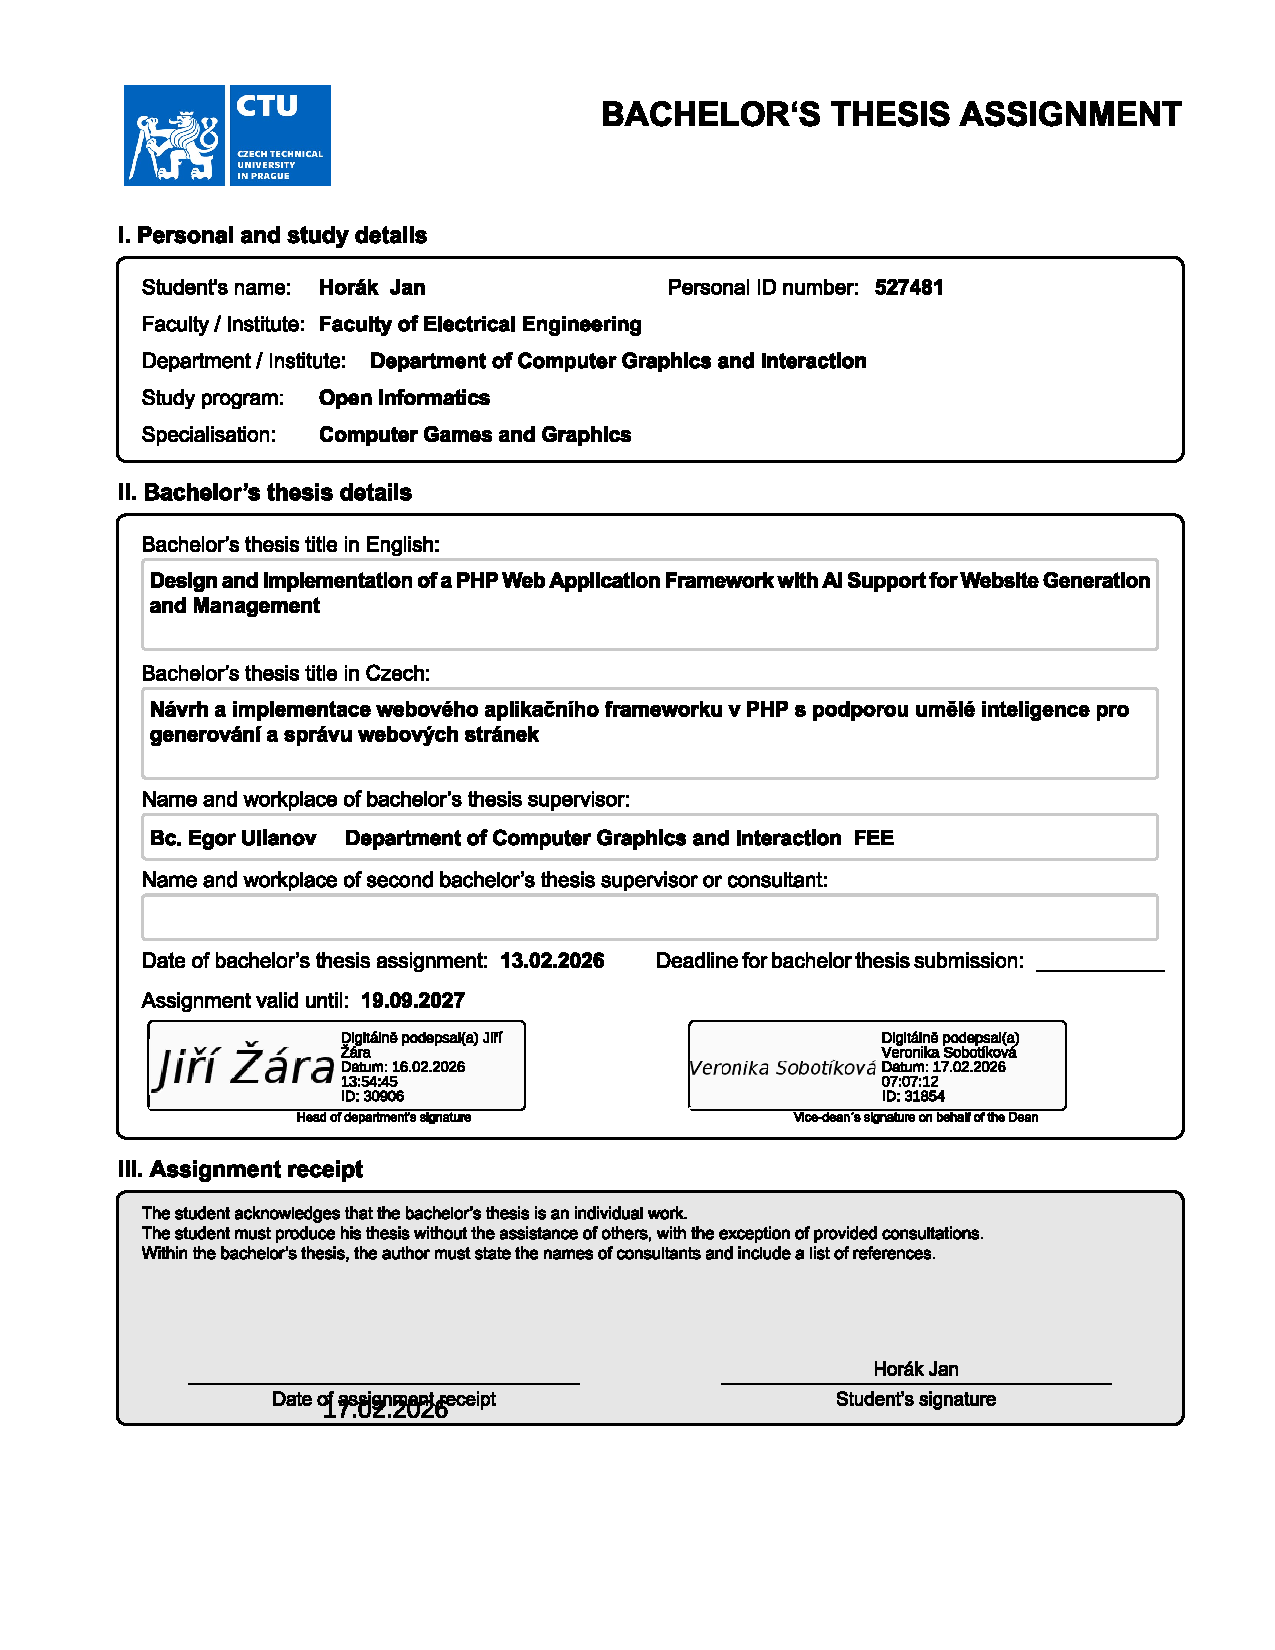
\includepdf[pages=-,pagecommand={},width=\paperwidth]{zadani.pdf}
    
\includepdf{prohlaseni}

    \clearpage

    \section{Introduction}\label{sec:introduction}
Building a feature-complete full-stack framework requires a strong architectural foundation.
However, an emphasis on rapid feature implementation often leads to compromises in architectural design.
This contributes to the perception that the architectural complexity of modern frameworks often exceeds the requirements
of their intended functionality.

The goal of this thesis is to design and implement a full-stack web framework focused on ease of development,
extensibility, and AI generation tooling with minimal usage of third party code.
The framework aims to define an abstraction layers to combat the ever-increasing complexity of frameworks.
The intention is to make full-stack development faster and more straightforward.

\subsection{Tasks}\label{subsec:introduction-tasks}
To satisfy the goal, the thesis is divided into tasks:

\begin{itemize}
    \item Research on state-of-the-art solutions.
    \item Study use cases and user stories.
    \item Design extensible full-stack framework architecture.
    \item Implement the core framework components, including content rendering, routing, database model abstraction,
        multilingual support, and forms.
    \item Develop administrative system for managing user configuration and management of user-generated content.
        This includes managing content web pages, files, localization, user roles, and privileges.
    \item Develop an editor subsystem capable of creating, manipulating, and deleting components.
    \item Implement AI generation foundation capable of generating static webpage templates, components for the editor, translations, code documentation.
\end{itemize}

\subsection{Hypothesis}\label{subsec:introduction-hypothesis}
This thesis proposes multiple hypothesis:

\begin{itemize}
    \item Unified and convention-driven an abstraction layer can streamline full-stack development.
    \item Implementing a framework without using third party code requires more effort upfront but pays off in ease of feature creation.
    \item Achieving robust architecture involves minimizing reliance on third-party libraries.
    \item AI generated content can drastically decrease time in content creation, but the system is brittle and still has a learning curve.
\end{itemize}


    \clearpage

    \chapter{State of the Art}\label{ch:state-of-the-art}
This section presents an overview of existing approaches and technologies.

\subsection{Technical terminology}\label{subsec:techical-research}
This subsection provides context on some of the terms this thesis uses.

\subsubsection*{CMS}\label{subsubsec:cms}
Content Management System is type of software that provides simple interface to create, manage, and publish digital
content without using a programming language~\parencite{oracle_cms}.
The software must provide sufficient tools for management of large datasets from different sources such as Social Media,
Internet of Things, and other~\parencite{kandepu_cms}.

\subsubsection*{AI}\label{subsubsec:ai}
In this thesis the terms LLM and AI are used interchangeably and both refer to software that returns text response from natural language request.
Large Language Models are transformer-based language models that are pre-trained on web-scale corpora.
These models are capable of obtaining world knowledge, generating code, following instructions, self-improve, and other~\parencite{minaee2025_llm_suvey}.
The proposed solution works with LLMs to generate structured text responses~\parencite{cloudflare_llm}.
LLMs can be simplified to a function that takes text input written in natural language and returns structured text response,
which can include parts written in natural language.

\subsubsection*{Framework}\label{subsubsec:framework}
Represents a large code base on which multiple developers collaborate~\parencite[6]{rahman2011}.
The code is structured for maintainability, reducing repetition, and onboarding new developers.
Frameworks give strong starting point for problems in target domain and handle common functionality for the domain.

\subsubsection*{Library}\label{subsubsec:library}
Libraries are collection of reusable software components for given domain.
The software components defined in library may be classes or procedures~\parencite[sec.~2.2, p.~8]{wegner1990}.
Libraries are not used until their functionality is explicitly called.
On the other hand, frameworks provide starting point and directly call user code.

\subsubsection*{Full-stack Web Development}\label{subsubsec:fullstack-web-development}
The Web development can be simplified into two distinct parts, back-end and front-end code.
Back-end code implements business logic on the server, which includes, but it is not limited to request handling,
file serving, database communication, and server side rendering.
Front-end code is served to the user as HTML, CSS, and JavaScript files that are then parsed and executed in the browser.
Full-stack developer works on both front-end interfaces and back-end procedures~\parencite[Full-stack Web Developer]{w3schools_fullstack}.

\section{Comparison of Existing Platforms}\label{sec:comparison-of-existing-platforms}
This section compares two widely used web platforms, WordPress and Squarespace.

\subsection{WordPress}\label{subsec:wordpress}
WordPress~\parencite{wordpress} is a widely adopted open-source content management system written in PHP\@.
It is flexible through its plugin and theming ecosystem.
The platform is open-source, which enables the developers to modify the core behavior if needed.

The primary advantages of WordPress include:

\begin{itemize}
    \item High flexibility due to being open-source.
    \item Large ecosystem of plugins and themes.
    \item Strong community support and documentation.
\end{itemize}

Excessive plugin usage may introduce inconsistent behavior or even produce security problems.
However, this flexibility comes at the cost of architectural complexity, which is partially addressed by code comments
and in-depth documentation.

From a developer perspective, WordPress is powerful but suffers from complex architecture accumulated over the years
of development~\parencite{wordpress_docs_rest}.

\subsection{Squarespace}\label{subsec:squarespace}
Squarespace~\parencite{squarespace} is a proprietary, fully hosted website builder focused on ease of use and visual design.
Even though Squarespace is closed-source system, it provides viable plugin system.

It may seem like closed-systems are more secure over the open-source projects.
However, this is not necessarily the case.
When security flaw is found in open-source system it is either fixed before it has a chance to be exploited
or the issue is fixed before it can negatively impact large number of users.
For example, the backdoor in xz Utils was identified through external analysis from third-party developer,
whose code depends on the library~\parencite{cve_2024_3094}.
This is the reason why the thesis proposed solution is open-source.

The main advantages of Squarespace include:

\begin{itemize}
    \item Fast setup and deployment.
    \item Integrated hosting and maintenance.
    \item Consistent user experience and stability.
    \item Minimal technical knowledge required.
\end{itemize}

The primary limitation of Squarespace is restricted extensibility of the core systems.
Developers cannot access the underlying backend architecture to host the websites on their own servers or to modify
core behavior.

Squarespace design philosophy prioritizes end users over developers,
which is reflected by the closed-source nature.
This makes it well-suited solution for less tech-savvy users, but lacks in flexibility for developers.

\subsection{Platforms Comparison Summary}\label{subsec:platforms-comparison-summary}
WordPress emphasizes openness and extensibility but suffers from architectural complexity.
Squarespace prioritizes simplicity but lacks customization needed for developers.
From a usability perspective, the Squarespace website editor is easier to use than the one WordPress provides.

Neither platform fully satisfies the requirements of a system that aims to provide:

\begin{itemize}
    \item Strong foundational architecture and modern code base.
    \item Full control over backend behavior.
    \item Extensibility without dependency-heavy ecosystems.
\end{itemize}

The thesis solution positions itself between these two approaches:
maintaining developer control and being open-source project similar to WordPress
while providing easy to use User Interface like the one Squarespace defines.


\subsection{Comparison of Existing Frameworks}\label{subsec:comparison-of-existing-frameworks}

\subsection{Object-Relation Mapping}\label{subsec:object-relation-mapping}
Many web applications needs to persistently store and retrieve data.
This is most commonly solved by connecting to a database, most commonly relational database.
While PHP includes standard way to connect to the database via PDO or other methods,
these solutions only address connection management, statement execution, and data retrieval using native SQL syntax.
Developing in this environment is prone to introducing bugs and vulnerabilities.

Object-Relational Mapping (ORM) creates Object-Oriented mappings for common queries, this decision, enables developers
to write code using the same paradigm as the rest of the application, while harnessing modern development toolkits for
code suggestions and encourage natural exploration of SQL through APIs.

Using ORMs may be suboptimal for~\parencite{orm}:

\begin{itemize}
    \item Performance
    \item Working with complex queries
    \item Using advance features beyond database queries
    \item Accessing different sources of data
\end{itemize}


\subsection{Large Language Models}\label{subsec:large-language-models}
Generalized language model was created from the demand for tasks with increasing complexity in natural language.
These tasks may include translation, summarization, information retrieval, code generation, and many more~\parencite[2]{naveed2025llm}.
Large Language Models are only subset of the field called Artificial Intelligence specialized in natural language processing.

The first models in natural language processing used rule-based techniques dominant in the 1950s and statistical models
in the 1980s.
The idea of Artificial Neural Network existed in the 1940s but hasn't seen much development.
These models were mainly used for binary classification, but they lacked the understanding of textual context
to deal with complex tasks~\parencite[History of Large Language Models]{raiaan2024llm}.

Large Language Models can be dissected into components each providing crucial functionality
~\parencite[Background of Large Language Models]{raiaan2024llm}:

\begin{itemize}
    \item Tokenization - The initial text is parsed into a sequence of tokens such as characters, symbols, parts of words, full words, parts of sentences.
        The main algorithms used in tokenization include WordPiece, UnigramLM, and Byte Pair Encoding.
    \item Attention - This mechanism improves performance of the models and is responsible for figuring out representation
        of input sequences and linking between tokens in the sequence.
    \item Activation Function - The function gives Large Language Model the ability to learn non-trivial concepts.
        Some of the activation functions are ReLU, GeLU, and other GLU variations.
    \item Normalization layer - Essential part in Large Language Model's convergence rate and improves stability during training.
        Some of the approaches are DeepNorm, RMSNorm.
    \item Data processing - Important part of the training process is general data processing.
        This ensures that the data is filtered for quality, de-duplicated, and removes personal data,
        which could lead to privacy concerns.
\end{itemize}

Usage of Large Language Models for generative or transformative purposes leads to ethical problems.
The organization should be transparent about the extent of AI usage in their works
to ensure expectation about quality of the provided service~\parencite[Ethical and Legal Considerations in AI Translation]{ablaikhan_translation_ai}.

\subsubsection{Translation}
Recent advances in Large Language Models have significantly improved the quality of translations.
Unlike traditional statistical or rule-based translation systems that are built on task-specific architectures,
Large Language Models are trained on large-scale multilingual dataset gives the ability to understand the textual context
and translate it accordingly to the meaning.

Classic GPT-based models excel at producing naturally sounding translations and are not limited to a few phrases,
which gives them ability to translate entire documents while preserving context.
Where human post-editing is still needed is for idiomatic phrases, ambiguous phrases, or translating words with multiple meanings.
Since Large Language Models are probabilistic their output can be different for the same sample of text when one output is strongly desired.
This probabilistic nature also introduces biases from training data,
particularly found in gendered languages and when translating sensitive topics~\parencite[Quality of AI Translations: Successes and Gaps]{ablaikhan_translation_ai}.
Models can be fine-tuned in prompt to translate the text in certain ways,
these translations are closer to transformation of a text and human intervention is needed to check for concept preservation.

The use of Large Language Models for translation introduces ethical and legal concerns.
Translations are derivative works, meaning that copyright of the original content must be respected,
even when Large Language Models is used for translation.
The user or organization using the translation tool is responsible for correcting translation mistakes introduced by the tool.

Current systems are efficient at dealing with routine translation tasks, such as translating phrases without context,
basic text, or structured text.
However, the same system still need human surveillance to meet the quality standards of translations~\parencite[AI vs. Human Translators: Can AI Replace Them?]{ablaikhan_translation_ai}.

\subsubsection{Code Generation}
Recent advances in Large Language Models have significantly improved the quality of code generations.
Code generation tasks are defined as generating code that performs the actions described in a given specification.
The description can be written as natural language prompt or introduce domain specific pseudo-language.

Large Language Models generate code by analyzing vast code bases in their training dataset~\parencite[AI Models and Techniques for Code Generation]{khade2025review_of_llm_code}.

Some of the common tasks may include~\parencite[Introduction]{chen2024survey_codellm}:

\begin{itemize}
    \item Prompt to executable code - The process of converting a natural language request into executable code.
        The generated code can be of different types: a small procedure with a well-defined functionality (e.g., a sorting algorithm),
        an architectural component implementing logic for a specific domain (e.g., a custom collection),
        or an executable script for an application or an operating system shell.
    \item Interpolating code templates - The prompt consists of mostly finished code snippet and description how to fill
        in the holes from context.
        Potential usage may be found in translation of UI templates.
    \item Refactoring existing code - The input includes the source code to be refactored and additional context.
        The context may include more source code or prompt describing the architectural ideas.
        The input also includes how the given code should be transformed.
        It is expected that the output is executable code, which interface and functionality is kept the same as the original code.
    \item Test case generation - The input includes the source code to be tested, additional context, and testing framework/library.
        The output are test cases validating the performance of the code in edge case situations and correctness in expected situations.
\end{itemize}

The usage of AI for code generation enables the developers to offload repetitive tasks, and they can focus on architectural design,
critical optimization problems, and other demanding tasks.
The shift from pure coding jobs to AI-assisted software engineering has reshaped the job market.
This development raises concerns about job displacement and changing demands for software developers~\parencite[Changes in Software Engeneering Job Roles]{khade2025review_of_llm_code}.

\subsubsection{Code Documentation}




    \clearpage

    \chapter{Use cases}\label{ch:use-cases}
The goal, of this section, is to clarify how users interact with the system
and how the core features solves real-world problems.

\section{User stories}\label{sec:user-stories}
Users, that are developers, are categorized by the level of their expertise.
For each user category different user story is created and analyzed.

More about the template used for the used stories can be found here~\parencite[User story template and examples]{atlassian_user_stories}

\subsection*{US1: Beginner Web Developer}
As a beginner web developer,
I want access to higher-level abstractions compared to the default PHP API,
so that I can easily build functional web applications.

As a beginner web developer,
I want features that support rapid prototyping,
such as imperative route declaration, simple database models, and intuitive content rendering,
so that I can quickly implement less complex systems.

As a beginner web developer,
I want to work with simple and transferable concepts,
so that I can apply the knowledge across different projects and technologies.

\subsection*{US2: Intermediate and Expert Web Developers}
As an experienced full-stack developer,
I want a framework that builds upon low-level technologies,
so that I can leverage my existing knowledge of these technologies and learn the framework faster.

As an experienced developer,
I want predictable architecture and reusable components,
so that I can efficiently develop and maintain complex systems.

As an experienced developer,
I want the ability to customize default behavior,
so that I can mold the system to project requirements easily.

As an experienced developer,
I want access to well-documented clean code and debugging utilities,
so that I can understand, troubleshoot, and extend the system effectively.

\subsection*{US3: Tooling and Library Developer}
As a tooling or library developer,
I want the framework to be highly modifiable,
so that I can build custom tools and libraries.

As a library developer,
I want access to application and external databases,
so that I can develop data-driven features.

As a tooling developer,
I want the ability to define sandboxed routing trees,
so that I can provide isolated functionality and not depend on project's structure.

As a tooling or library developer,
I want readable and well-structured source code,
so that I can understand and extend the framework efficiently.

\subsection*{US4: Administrator}
As an administrator,
I want to manage user groups and assign privileges,
so that I can control access to different parts of the system.

As an administrator,
I want to restrict access to sensitive system features such as system settings and user privilege management,
so that critical functionality is protected from unauthorized changes.

As an administrator,
I want to manage uploaded files,
so that the structure is properly organized.

As an administrator,
I want to manage languages and translations,
so that the User Interface can be localized when deployed.

As an administrator,
I want to manage system-level configurations including users, groups, settings, and PHP configuration
so that I can maintain and monitor the system effectively.

As an administrator,
I want to view AI-generated documentation and request documentation for source files,
so that I can maintain up-to-date technical documentation.

\subsection{Primary Use Cases}\label{subsec:primary-use-cases}
The primary use cases of the framework focus on simplifying web development and removing unnecessary boilerplate.

\subsubsection*{UC1: Define a Database Table}
A developer defines a new database table, after which the framework automatically infers table querying operations (first, all).
From the defined database table schema the framework can create automatic grid template or simple form for creating or updating
records of the table.
The framework's admin package is able to infer logic for simple Create, Read, Update, and Delete operations with web-based UI\@.

\subsubsection*{UC2: Create a Webpage Using Component-Based Editor}
A developer composes a web-page by assembling components such as headers, paragraphs, lists, images,
or other custom-built components.
The editor stores metadata required for rendering and persists the final structure on the server.
If desired component is not implemented it can be easily created with AI-Generation component.

\subsubsection*{UC3: Responding to a Request}
A developer renders content as a response using the framework's abstraction layer that unifies routing, rendering, and database access.
This reduces the need for manual wiring between layers while providing the benefits of decoupled logic for each layer.

\subsubsection*{UC4: Extend Default Form Generation}
A developer modifies the automatically generated form by overriding the default form controls or injecting custom controls.
The framework preserves the simplicity of automatic forms while allowing targeted customization.

\subsubsection*{UC5: Custom Static Webpage}
A producer wants to draft out a simple static webpage without touching code, but providing a sample for the developer
team.
The framework comes with out-of-the-box solution for AI generated static webpages.

\subsubsection*{UC6: Automatically Generate Translations for Static Text}
A developer defines phrase in template and in the administration dashboard users with privileges to access translations
can write translate phrases directly or off-load the translation to an AI\@.

\subsubsection*{UC7: Group Privileges Assignment}
An administrator creates new group for users and assigns fitting privileges.
This way users can log in to the administration dashboard and work on parts of the system assigned to them and
ensures that unauthorized users cannot access critical parts of the system.


    \clearpage

    \section{Requirements}\label{sec:requirements}
This section defines the functional and non-functional requirements.

\subsection{Functional Requirements}\label{subsec:functional-requirements}
These requirements specify how the system implements core systems, AI tooling, and expected behavior from users.

\subsubsection{Framework Requirements}
\begin{itemize}
    \item FR1: The framework must provide a deterministic routing system.
    \item FR2: Routing system must support common HTTP methods.
    \item FR3: Routing system must be modular, such that part of the routing tree can be moved to different branch
        and all the bindings must work as expected.
    \item FR4: The framework has the ability to automatically infer CRUD operations for database tables.
    \item FR5: Models must map database columns to properties without extra boilerplate.
    \item FR6: The framework must provide form-handling subsystem.
    \item FR7: The system has the ability to automatically infer forms based on model structure.
    \item FR8: The framework must provide a component-based editor capable of creating and maintaining webpages.
    \item FR9: Editor components must be rendered on client from provided structure.
\end{itemize}

\subsubsection{AI Generation Requirements}
\begin{itemize}
    \item AIR1: The system must include an AI-powered translation unit capable of translating static text and text templates for supported languages.
    \item AIR2: The framework must support generating new editor components.
    \item AIR3: Users must be able to request AI-generated static webpages from natural language prompt.
    \item AIR4: The system must provide AI-documentation from its own source files.
    \item AIR5: The system must include website structure generation of pages and their templates.
\end{itemize}

\subsection{Non-Functional Requirements}\label{subsec:non-functional-requirements}
These requirements specify how the whole system behaves rather than addressing specific functionalities.

\begin{itemize}
    \item NFR1: The system must prioritize ease of development, readability, and extensibility.
    \item NFR2: New features, components, and templates must be easy to add and maintain.
    \item NFR3: The framework must perform efficiently enough for small-to-medium projects.
    \item NFR4: All core features must be implemented with minimal reliance on third-party libraries.
    \item NFR5: The code must follow the conventions defined by the framework’s philosophy.
    \item NFR6: The framework's systems must follow a unified design approach.
\end{itemize}


    \clearpage

    \section{System Design}\label{sec:system-design}
This section describes how the system works without going into the implementation details.
Painting the whole system as a black-box implementation, the interface is known, but the underlying implementation is not.

\subsection{Design Goals}\label{subsec:design-goals}
The primary objective of the system is to provide a flexible environment for full-stack development.
The design emphasizes simplicity and ease of integration, allowing the components extended easily.

The key design goals are:
\begin{itemize}
    \item Simplicity - The system interface is simple and similar and the implementation of programming patterns is consistent.
    \item Modularity - The system is divided into components.
    \item Extensibility - New functionality can be added to existing components.
    \item Automation - Repetitive development tasks should be automated with AI if possible.
    \item Transparency - The system should expose clear interface for each component.
\end{itemize}

These goals reflect the prototype nature of the system, which aims to explore automation of common full-stack development tasks.

\subsection{System Overview}\label{subsec:system-overview}
The system is designed as a collection of loosely coupled services that operate on shared dataset.
At a high level, the system accepts requests and based on them generates appropriate responses.
All services operate independently communicating trough common interfaces.

The system adopts a black-box design approach, where each component is defined by its usage interface and expected behavior.
This allows the system to be heavily modified if needed and new features to be added easily.

\subsubsection{Routing}
The routing component takes care of path to executable action translation, which includes request and response creation,
action interface definition, and dispatching actions in deterministic order.
The component exposes functions that mount different types of endpoints to specified route.
Route is defined as dynamic template for request paths which removes duplicity and enables variable routing.

\subsubsection{Database Connection}
The system aims to support connections to multiple databases of varying types, such as SQL or graph-based.
The Database Connection acts a specification and guideline to implementing connections to each database type.
Each type of database is required adhere to the specification and implement its own type of connection interface including
Object-Relation Mapping (ORM) for querying data.

\subsubsection{Asset Loading}
The system is designed for full server-side-rendering as well as granular UI streaming.
To satisfy this claim the system includes component for asynchronous asset loading called SideLoader.
SideLoader exposes importer interface specifying supported file types, passing files to be imported,
and handling import events.
The importer is used to generate one blob of all the assets which is sent to the frontend where it is parsed and incorporated.
The prototype defines importers for CSS and JavaScript.
SideLoader is coupled with extension that implements HTML content streaming through custom HTML attributes and enables
the extension to load assets the same way as if the whole page was rendered on the server.

\subsubsection{Translation}
User interface implementations include static text that is not editable by editors, although it requires translation.
The component defines an interface in which the text serves as a key for corresponding translations.
Using the administration dashboard, editors can find this text and either provide translations manually or generate them using AI\@.

\subsubsection{Administration}
Administration dashboard is a collection automatic procedures that includes: form extraction from database model,
table listing of records from collection, creation of new records, and editing existing records.
The dashboard also provides system utilities and for the developers web view of test results.

The administration dashboard includes component-based widget editor for managing website content.
The editor is capable of generating new widgets from AI prompt.

\subsubsection{Testing}
The testing component aims to provide clear interface for simple unit testing with output rendering to enable viewing results
in web view or analysing the results through JSON data representation.


\subsection{System Data Flow}\label{subsec:data-flow-and-integration}
All components have access to the databases that act as a shared representation of project data.
There a few miscellaneous objects for exposing globally constant values.

\begin{figure}[H]
    \centering
    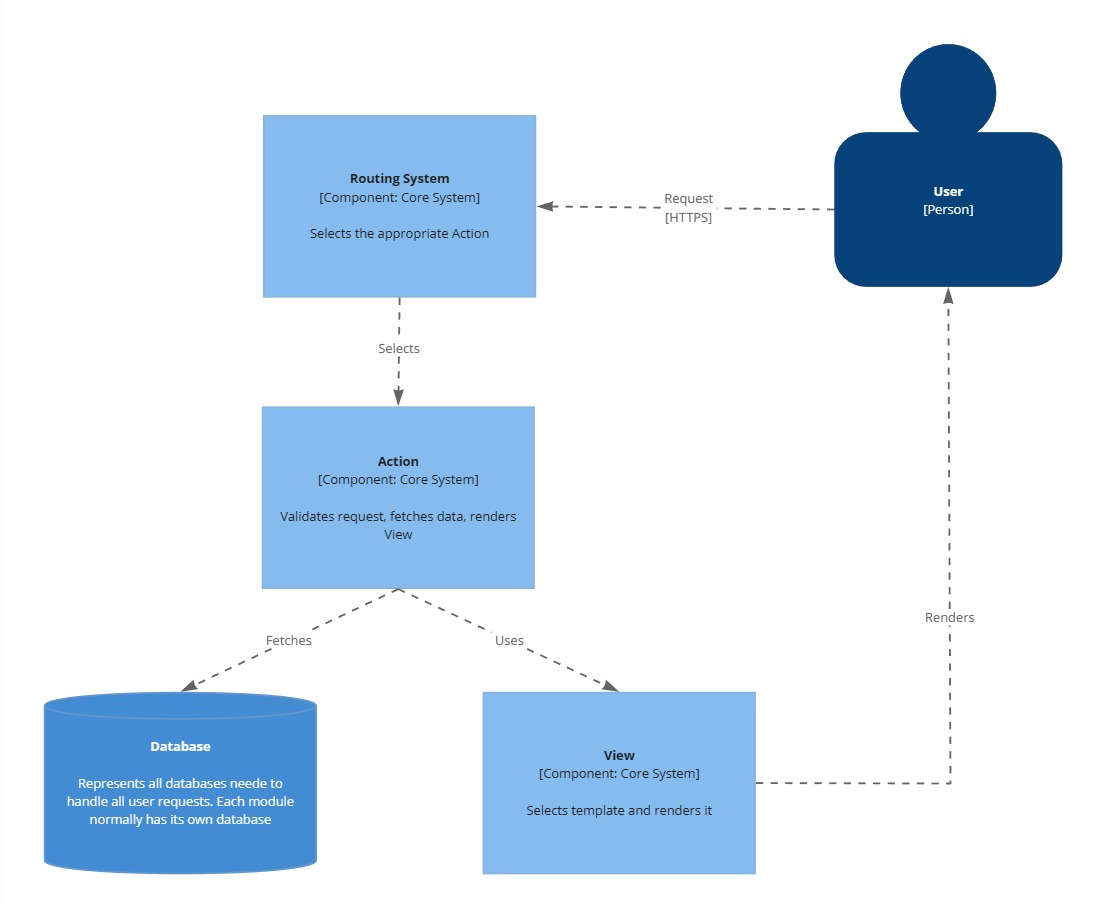
\includegraphics[width=0.75\linewidth]{images/c4-diagram}
    \caption{Architecture}
    \label{fig:architecture}
\end{figure}

The typical workflow consists of the following steps:

\begin{enumerate}
    \item Creation of request specific data objects and database connections are established.
    \item Execution of actions responsible for handling the request.
    \item Actions run business logic using database records or delegate processing to other system components.
    \item Response is aggregated and rendered in desired format to the user.
\end{enumerate}

\begin{figure}[H]
    \centering
    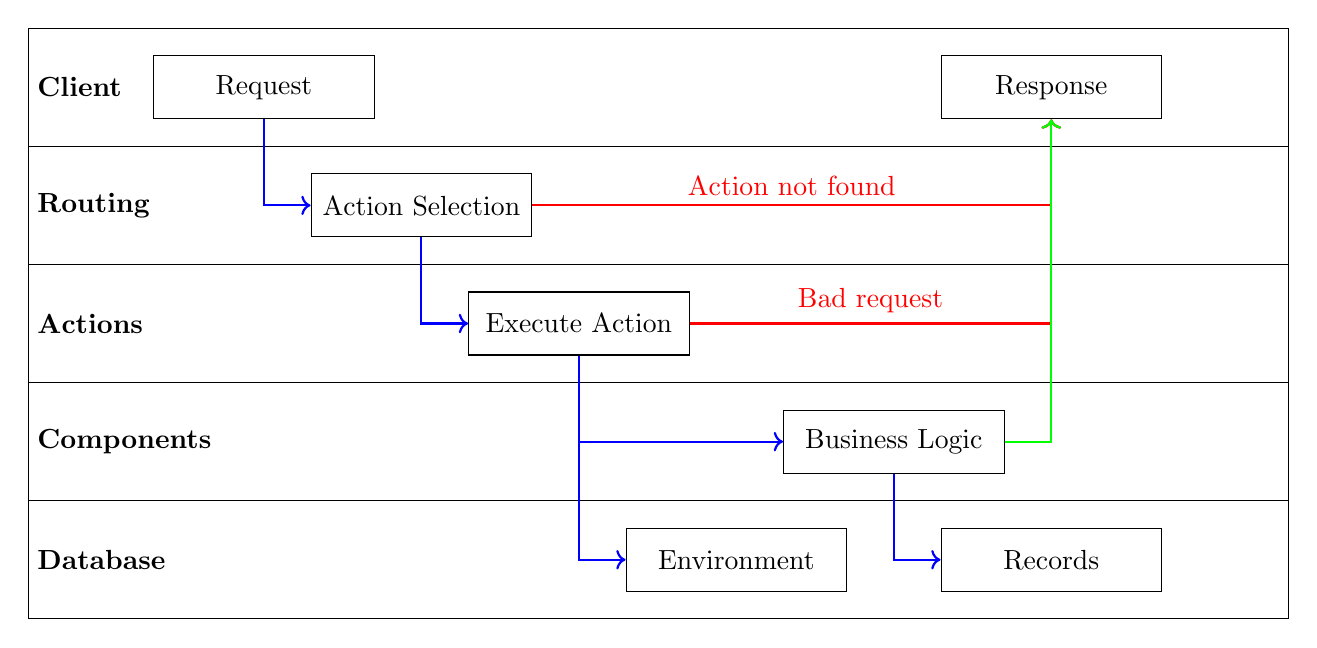
\begin{tikzpicture}
        [
        node distance=2.5cm,
        lane/.style={draw, minimum width=16cm, minimum height=1.5cm, anchor=west},
        activity/.style={draw, rectangle, minimum width=2.8cm, minimum height=0.8cm},
        arrow/.style={->, thick}
        ]

        \node[lane, label={[anchor=west]west:\textbf{Client}}] (client) at (0,4) {};
        \node[lane, label={[anchor=west]west:\textbf{Routing}}] (routing) at (0,2.5) {};
        \node[lane, label={[anchor=west]west:\textbf{Actions}}] (actions) at (0,1) {};
        \node[lane, label={[anchor=west]west:\textbf{Components}}] (components) at (0,-0.5) {};
        \node[lane, label={[anchor=west]west:\textbf{Database}}] (db) at (0,-2) {};

        \node[activity] (req) at (3,4) {Request};
        \node[activity] (response) at (13,4) {Response};

        \node[activity] (route) at (5,2.5) {Action Selection};

        \node[activity] (action) at (7,1) {Execute Action};

        \node[activity] (logic) at (11,-0.5) {Business Logic};

        \node[activity] (env) at (9,-2) {Environment};
        \node[activity] (query) at (13,-2) {Records};

        \draw[arrow, blue] (req) |- (route);
        \draw[arrow, blue] (route) |- (action);
        \draw[arrow, blue] (action) |- (logic);
        \draw[arrow, blue] (action) |- (env);
        \draw[arrow, blue] (logic) |- (query);

        \draw[arrow, red] (route) -| node[pos=0.25, above] {Action not found} (response);
        \draw[arrow, red] (action) -| node[pos=0.25, above] {Bad request} (response);

        \draw[arrow, green] (logic) -| (response);

    \end{tikzpicture}
    \caption{System Request Processing}
    \label{fig:system-request-processing}
\end{figure}

This pipeline-oriented design enables skipping defined steps if needed.

\subsection{Summary}\label{subsec:summary}
The proposed design emphasizes simplicity, abstraction, and extensibility.
Designing modern systems requires solving domain-specific problems while satisfying system constraints.
Simplicity and extensibility are two constraints that work against each other.
Simple solutions suffer from architectures that are difficult to extend, while extensible systems are overly reliant
on abstraction, leading to confusing APIs.
Implementing a complex design is an act of balancing between rigid architecture and convoluted abstractions.

    \clearpage

    \section{System Architecture}\label{sec:system-architecture}
This section describes the challenges encountered during implementation of proposed design and techniques used to solve them.
The design expects full independence between system's components, in practice, some coupling emerges due to accessing shared
resources, execution order, communication, and code reuse.

The architecture follows a hybrid approach combining:
\begin{itemize}
    \item Centralized data access through shared database connections.
    \item Globally accessible Request and Response objects.
    \item Interface-driven communication between components.
    \item Developer constants are defined in respective classes serving static key-value look-up tables.
\end{itemize}

This approach provides easily accessible datasets, that are needed in all parts of the system.

\subsection{Component-Level Architecture}\label{subsec:component-architecture}
This section addresses challenges faced during implementation of each component.



\subsubsection*{Routing}
The routing mechanism is responsible for mapping request paths to actions.
During implementation, several challenges arise:

\begin{itemize}
    \item Internal structure - The initial solution used naive tree implementation, which lacked proper edge definitions.
        This problem manifested through convoluted rules during traversal, that made adding more features increasingly difficult.
        The structural problem was solved by proper implementation of general graph collection and using modified graph
        traversal algorithms.
        Implementation of proper graph collection enabled adding data to connections for reasons beyond routing.
        Simplest example of this feature are menu routes that contain route definition, labels for each segment, and optional icon.
    \item Ambiguity of routes - Routes are dynamic templates for request paths including static and variable parts of a path's segment.
        Segments are marked by their type, which holds precedence rules.
        Search results are aggregated and sorted by the precedence rules to ensuring deterministic order of search results.
    \item Route template evaluation - The system may include hundreds of routes and each of them may be evaluated during search.
        Each route is parsed into intermediate object representation by custom-made route compiler using the compiler architecture~\parencite{appel2000_compiler_design}.
\end{itemize}

Examples of routes:
\begin{verbatim}
    / - Get current node.
    /** - Match all segments after **. This definition is
        least descriptive thus it has the lowest prescedence.
    /foo - Match static "foo"
    /[foo] - Save first segment as "foo" variable
    /foo/[bar] - Match first segment as static "foo"
        and save the value of second segment to the "bar" variable
    /foo/bar-[id] - Match first segment as static "foo"
        and match the second segment as "bar-"
        and save the remainder to the "id" variable
\end{verbatim}



\subsubsection*{Database Layer}
Tha main challenge when developing the database abstraction, was providing clear and expressive configuration.
The implementation of the configuration had to be performant enough to be accessed multiple times for each outgoing query.
Working with JDBC (Java Database Connection) library inspired the code with metadata approach using class attributes.
The database layer abstracts tables through PHP classes.
Each model declares its database connection, associated table, and table columns through PHP attributes.

Example of mapping users table to the User class:
\begin{verbatim}
    #[Database(App::DATABASE)]
    #[Table('users')]
    class User extends Model {
        #[Column('id_user', Column::TYPE_INTEGER, primaryKey: true)]
        protected int $id;

        #[Column('name', Column::TYPE_STRING)]
        protected string $name;
    }
\end{verbatim}

From this definition, the system is capable of:

\begin{itemize}
    \item Executing standard fetch queries (first, all, fromId, and count number of records for given condition).
    \item Creating new User records in database.
    \item Updating a User record.
    \item Deleting a User record.
\end{itemize}

All Query function uses parametrized query if needed.
For example to remove record from users table with id 4.

\begin{verbatim}
    // Creates DeleteQuery object
    $query = Sql::delete('users');

    // DELETE query is requred to have where clause
    // Query::infer automatically infers the parameter type (TYPE_INTEGER)
    $query->where(Query::infer('id_user = ?', 4));
\end{verbatim}

If the developers use provided Query classes correctly there shall never be SQL injection.
The Database Layer provides default fetching functions first and all which uses the same Query object.
Default implementation of first and all functions return one or many instances of model objects.
Fetch function uses the projection parameter to add developer defined SQL query projection optimization.
Implementation of Database Layer does not use the \("\)SELECT *\("\) projection variant although SelectQuery objects
uses it if projection is not set.
Not defining projection for SelectQuery is not encouraged.

\begin{verbatim}
    // Returns record with the id 4
    // populating all column properties on the User object
    // SELECT id_user, name FROM ...
    User::first(where: Query::infer('id_user = ?', 4));

    // Returns record with the id 4
    // populating only columns defined in projection array
    // SELECT name FROM ...
    User::first(
        projection: ['name'],
        where: Query::infer('id_user = ?', 4)
    );

    // When using select query directly projection
    // may not be set and thus the * is used.
    // Uses SELECT * FROM ...
    $query = Sql::select('users')
        ->where(Query::infer('id_user = ?', 4));
\end{verbatim}

Defining custom ORM database interface provides control how the features are implemented and integrated into the system.



\subsubsection*{Asset Loading (SideLoader)}
The SideLoader component introduces asynchronous asset handling, which complicates an otherwise synchronous server-side
rendering pipeline.

Observed issues:
\begin{itemize}
    \item Context independent importing - The core problem that SideLoader addresses is importing assets for code that
        is injected into the HTML page during rendering or loaded asynchronously when HTML components are fetched through AJAX\@.
        The solution uses unique identifier for each asset file and endpoint that accepts list of identifiers and returns asset blob.
        During rendering all assets are caught by the corresponding import functions and list of identifiers is generated.
        If response includes HTML head element, the import call to the endpoint is injected into the head otherwise
        the list is passed through custom HTTP header in the response and JavaScript injects import element into the head.
    \item Dependency resolution - For the sake of simplicity, the dependencies are not resolved and all assets need to imported
        explicitly.
    \item Debugging - JavaScript files requires certain order of importing the scripts.
        Static loading for all pages of commonly used libraries solves most of the issues with incorrect import order.
        For the remaining cases, custom events are dispatched when code is imported.
\end{itemize}



\subsubsection*{Translation System}
The translation system uses static text as keys, which simplifies integration but introduces constraints:

\begin{itemize}
    \item Coupling - If default language is changed all the UI text need to be changed as well because the static text are written
        in default language.
        If request requires the default language the the system returns the static text to improve performance.
    \item Refactoring - When refactoring the static texts the system creates new database records.
        The system can not determine unused keys, and so they are left in database showing in administration dashboard.
    \item Ambiguity - Each key requires translation group to resolve ambiguous keys.
        The group-key pair should always correspond to only one static text.
\end{itemize}

Example usage of the translation system:
\begin{verbatim}
    // MyUiComponent.php
    class MyUiComponent implementes View {
        // UI rendering code ...

        // Provides shorthand methods for static text translation
        use LexiconUnit;

        public function __construct() {
            $this->setLexiconGroup("example.group");
        }
    }

    // MyUiComponent.phtml
    <button>
        <!-- Creates a new pairing: (exmaple.group and Submit) -->
        <!-- and searches for correct translation -->
        <?= $this->tr("Submit") ?>
    <button>
\end{verbatim}



\subsubsection*{Administration Interface}
The administration system automates CRUD operations based on database models.
While this reduces development effort, it introduces constraints:

\begin{itemize}
    \item Workflows - The administration dashboard handles simple CRUD well, but they lack data validation logic.
        If validation is required, then editor behavior needs to implemented.
        The editor behavior is solution to most common create/update feature requests.
        It supports custom form creation and on submit validation while editor takes care of form submission and model creating/updating.
    \item Database structure - It is limitation of the current system that it only works with built-in SQL connections.
        The problem is acknowledged but not addressed further.
    \item Grid - The current system supports custom grid rows definitions, but they have to be descendant of Model class.
        This means, if the row is composed of multiple database tables either each rows explodes into multiple database calls
        during rendering or new abstract model needs to be implemented to wrap results of complicated select queries.
    \item Menu routes - The administration dashboard required side menu for navigation.
        Naive implementation of showing the route segment to the user would work, but it is not ideal for the user,
        since url paths do not support spaces and other special character.
        This problem was solved by implementing proper graph collection described in the Routing section.
\end{itemize}



\subsubsection*{Testing}
The testing component is designed for simplicity, but this simplicity leads to:

\begin{itemize}
    \item Complex testing scenarios - The current system does not support testing beyond simple unit tests.
    \item Implementation - The library used for testing is implemented naively and lacks in implementation quality.
    \item Manual inspection - The results of tests needs to be viewed on the administration dashboard and currently
        does not support running tests automatically and notifying about the results.
\end{itemize}

Example of simple unit tests using the library:
\begin{verbatim}
    // utils.php
    Sptf::test("match arrays", function () {
        Sptf::expect(Arrays::equal([], []))->toBe(true);
        Sptf::expect(Arrays::equal([1], [1]))->toBe(true);
        Sptf::expect(Arrays::equal([1], []))->toBe(false);
        Sptf::expect(Arrays::equal(["foo" => "bar"], ["foo" => "bar"]))
            ->toBe(true);
        Sptf::expect(Arrays::equal(["foo" => "bar"], ["bar" => "foo"]))
            ->toBe(false);
    });
    // Results: PASS 0.00s "match arrays" 5 assertions

    Sptf::test("reverse array", function () {
        $array = [0, 1, 2, 3, 4, 5, 6, 7, 8, 9];

        Sptf::expect([...Arrays::reversed($array)])
            ->compare(fn($a, $b) => Arrays::equal($a, $b))
            ->toBe(array_reverse($array));
    });
    // Results: PASS 0.00s "reverse array" 1 assertions
\end{verbatim}


\subsection{Data Flow and Execution Model}\label{subsec:architecture-data-flow}

Although the design suggests a clean pipeline, the actual execution model includes
additional complexity:

\begin{itemize}
    \item Implicit dependencies between components
    \item Shared mutable state through database connections
    \item Conditional execution paths based on runtime context
\end{itemize}

These factors make the system harder to reason about compared to the idealized
pipeline model.

\subsection{Cross-Cutting Concerns}\label{subsec:cross-cutting-concerns}

Several concerns affect multiple components simultaneously:

\begin{itemize}
    \item \textbf{Performance:} Abstractions introduce overhead, especially in routing
    and database access.
    \item \textbf{Consistency:} Shared data access increases risk of inconsistent state.
    \item \textbf{Scalability:} Tight coupling through shared resources limits horizontal scaling.
    \item \textbf{Debugging:} Indirect interactions between components complicate tracing errors.
\end{itemize}

These concerns highlight the gap between theoretical design and practical implementation.

\subsection{Architectural Trade-offs}\label{subsec:architectural-tradeoffs}

The implementation reflects several key trade-offs:

\begin{itemize}
    \item Simplicity vs. flexibility
    \item Abstraction vs. performance
    \item Automation vs. control
\end{itemize}

In many cases, decisions favor simplicity and rapid development over long-term
scalability and robustness, which is consistent with the prototype nature of the system.

\subsection{Summary}\label{subsec:architecture-summary}

The system architecture exposes the complexity hidden behind the high-level design.
While the design goals emphasize modularity and extensibility, the implementation
reveals constraints imposed by shared data, abstraction layers, and component interaction.

The resulting architecture represents a compromise between theoretical design
principles and practical feasibility, highlighting areas for future refinement.

    \clearpage

    \section{Using the Prototype To Create Websites}\label{sec:creation-process-of-websites}
This section focuses on explaining the process of setting up the prototype framework, RouteChasm~\parencite{github_routechasm}, and using it to create
three websites of varying types:

\begin{itemize}
    \item Personal - Chrome browser extension for widget-oriented New Tabs~\parencite{github_startuh}
    \item Corporate - Software Agency advertising their services, projects, and blog articles~\parencite{github_strata}
    \item Content-driven - Administrator curated repository of recipes and cooking related articles~\parencite{github_savora}
\end{itemize}

The websites are testing the following sections:

\begin{itemize}
    \item CMS components
    \item AI generation (Page Structure Generation, Article Generation, Static Page Generation, Page Component Generation, Documentation Generation)
    \item Development metrics (Requirement Coverage, Number of Manual Edits, Time to Publish, Responsiveness, and Basic SEO)
\end{itemize}

\subsection{PHP and MySQL}\label{subsec:php-and-mysql}
The recommended way to host the application locally is by installing Wampserver~\parencite{wampserver}.
Download the full version of Wampserver, this will include PHP server, MySQL server, and PHPMyAdmin to manage the MySQL server.
While installing the Wampserver you might need to install Visual C++ Redistributable Packages for your system which can
also be found on the Wampserver website.

After installing and running it, download cacert.pem file, and add absolute location to the file to the curl.cainfo field
in php.ini file.
This will enable the server side AI generation requests.

\subsection{Initial setup}\label{subsec:initial-setup}
For each website the following shell code was executed to create project directory, download the latest version of
the framework, and change the remote origin (GitHub repository).

\begin{verbatim}
    # Download the framework
    git clone https://github.com/CaptSiro/route-chasm.git <project-name>
    cd <project-name>

    # Remove project's git history (recommended through file explorer)
    rm -rf .git
    # Create the project's local repository
    git init

    # Push the framework to the origin
    git remote add origin <project-git>
    git add .
    git commit -m "Initial commit from RouteChasm"
    git branch -M main
    git push -u origin main
\end{verbatim}

Before the project is ready for local testing a few configuration files needs to be updated.
The .htaccess file routes all the requests to a singular file and the framework takes care of the individual request resolution.
By default, this file routes the requests to the file route-chasm/index.php but the real location of the index.php file
depends on where the project is located in relation to the web server's root directory.
Most of the time, the web server's root directory is the parent directory of the project.

\begin{verbatim}
    ...
    RewriteRule (.*) /<project-name>/index.php [QSA,END]
    ...
\end{verbatim}

Now, any incoming requests are handled but the framework lacks environment specific configuration.
By default, the framework tries to get all the configuration from the .env file.
The file is not provided in the framework repository, because it defines sensitive information, for example, root login details,
database user login, and api keys.
The .env file must be created and edited by hand.
The following .env template contains all the fields used by the framework with sample values.

\begin{verbatim}
    VERSION=1.0.2

    PROJECT=<Project-Name>
    PROJECT_LINK=<project-git>
    PROJECT_AUTHOR=<Project-Author>
    PROJECT_AUTHOR_LINK=<project-author-link>

    LANGUAGE=en-US
    DOMAIN_URL=<deploy-url>

    DATABASE_HOST=127.0.0.1
    DATABASE_NAME=routechasm
    DATABASE_USER=root
    DATABASE_PASSWORD=root

    ADMIN_LOGIN_PASSWORD=root

    OPENAI_KEY=<api-key>
    OPENAI_MODEL=gpt-4o-mini
\end{verbatim}

Login to the database manager (PHPMyAdmin recommended and preinstalled in Wampserver) and create new database.
Locate the src/core/sql/init.sql file and run it in the database.
This will create empty RouteChasm database.
To load in the database with data run the src/core/sql/export.sql file.
Each project includes its own export.sql file.

The framework is ready to be used.

\subsection{Implementation Specifics of Corporate Website Scenario}\label{subsec:implementation-specifics-of-corporate-website-scenario}
The Home directory provided by the framework does not include JavaScript file,
but the project homepage requires extra JavaScript functionality and thus home.js is created
and the functionality is implemented.
The template is edited to import the script file using SideLoader's Javascript::import() method and the homepage layout
is designed and implemented.



\subsection{Common Edits}\label{subsec:common-edits}
This section is going to address a few common changes, that can be applied to the framework.

\subsubsection*{Adding Meta Description to Homepage}
All pages created through administration dashboard include textarea to fill in meta description.
The homepage component is defined in src/components/Home/Home.php.
In the constructor the HtmlHead is created, and it includes function to add meta fields.
Adding description editable through web settings can be added this way:

\begin{verbatim}
    parent::__construct(
        new ContextAwareWebPage(
            // Save the HtmlHead to variable
            head: $head = new HtmlHead(...)
        )
    );

    $description = Setting::fromName(
        'project:homepage-description',
        // Create the setting if it is not defined
        true,
        // Default description
        '',
        // Makes the setting editable in admin dashboard
        [PROPERTY_EDITABLE => true]
    );

    $head->addMeta('description', $description->toString());
\end{verbatim}

\subsubsection*{Editing Homepage Button Behavior}
Locate the src/components/Home/Home.phtml template and edit the HTML of the page.
To add JavaScript functionality locate home.js in the same directory.
If the script file is created it needs to be created by hand and this line of code added to the template:

\begin{verbatim}
    // getRosource function locates the file
    // relative to the class definition of the $this object
    Javascript::import($this->getResource('home.js'));
\end{verbatim}

Edit the script to the needs and reload the page.
The changes should take place instantaneously.

\subsubsection*{Uploading Files}
Files can be uploaded via the administration dashboard.
The files are limited to pages created in dashboard and can not be used natively in homepage template.
Navigate to the Admin/File System/Files page and drag-and-drop your files on to the grid.
Drag-and-dropping is the only way to upload files to the system.

\subsubsection*{Changing Homepage Image}
Add images to the public/images directory, locate the src/components/Home/Home.phtml template, and create or edit the
desired HTML image element.
The images are accessible on url: <project-domain>/public/images/<image-file>

\subsubsection*{Creating Editor User}
Navigate to the System/Groups and create new group called Editors and fill out the privileges mapping.
Each checkbox corresponds to Resource and Action performed on the resource.
If the checkbox is checked it means that the group has privilege to perform the action on the resource.

Navigate to the System/Users and create new user.
When creating a new user, the Tag needs to be unique for the website.
Add the user into the Admin group which gives them the access to log into the administration dashboard
and the newly created Editor group defines all the actions the user can perform in the dashboard.



    \clearpage

    \section{Conclusion}\label{sec:conclusion}
The goal of this thesis is to design and implement a full-stack web framework focused on simplifying the development,
supporting extensibility, and integrating AI-Generation features.
One of the sub goals is to implement the framework with minimal usage of third-party code.
Currently, the prototype does not rely on external libraries or other frameworks, it uses internally developed libraries
and standardized PHP extensions such as curl, PDO, fileinfo, gd, and mbstring.
This fulfills the NFR4.

\subsection*{Hypothesis Evaluation}\label{subsec:hypothesis-evaluation}
The observations during implementation and evaluation results generally support the hypotheses proposed in Chapter~\ref{subsec:introduction-hypothesis}.

The scenarios demonstrated that unified and convention-driven abstractions simplifies the deployment of applications with varying types.
The built-in features enabled rapid deployment of smaller to medium-sized applications while supporting custom implementation if needed.
This and evaluation results qualitatively satisfy the NFR1.
The scenarios confirmed the usability of the tested systems and AI-Generated content.
The System Usability Scale evaluation of the prototype produced an average of 70, which makes the implementation acceptable.

Observations during implementation showed that minimizing reliance on third-party dependencies improved consistency
and streamlined integration of subsystems across the architecture fulfilling the NFR2,
although it increased the implementation time.

The evaluation results show that AI-Generated content decreases the time spent on content creation.
However, the evaluation confirmed the AI-Generated content requires manual verification and modification.

Due to the limited scope of the implemented prototype and smaller number of participants in evaluation,
the conclusion should be interpreted as observation rather than statistically validated result.

\subsection*{Requirements Evaluation}\label{subsec:requirements-evaluation}
The implementation observations and evaluation results indicate that the framework fulfills the majority of requirements.

The NFR3 requirement is perceived as partially satisfied based on qualitative evaluation.
During implementation and evaluation actions performed by the framework did not exceed the expect time to fulfill the request,
thus the framework is performant enough for small-to-medium sized projects.
However, no performance benchmarking was conducted.

\subsection*{Limitations of the Prototype}\label{subsec:limitations-of-the-prototype}
The thesis also identified several limitations of the current implementation.
Currently, some advanced features expected from modern full-stack framework require manual implementation.
These include on-demand user sign in, collaborative editing, e-commerce support, and general visual content editor.
Additionally, the implemented architecture favors solutions maximizing for simplicity, abstraction, and control.
For example, the closed user system simplifies administration but limits the usability in systems opened the public registrations.

\subsection*{AI-Generated Content}\label{subsec:ai-generated-content}
The AI-Generated content demonstrated usefulness for certain tasks, such as article content generation and phrase translation.
Although, the evaluation shows that AI-Generated outputs require manual verification and modification.
As a result, AI-Generation features should currently be considered a supporting tool for drafting purposes rather
than automated solution generation tool.

\subsection*{Future Work}\label{subsec:future-work}
Future Work should focus primarily on improving extensibility of the system, reducing manual implementations, and refactoring
outdated systems.
Potential improvements include replacement of component-based widget editor for general visual content editor,
support for modules, improvement of authentication system, refactoring the structure of the repository, and adding more
page templates such as contact page.
Additionally, conducting a larger-scale usability evaluation with framework-specific questions to identify the weaker parts of the system.

\subsection*{Final Thoughts}\label{subsec:final-thoughts}
Overall, the thesis shows that the implemented framework is usable for wide range of use cases and enables rapid deployment
of simple projects.
Although, the framework currently contains several limitations, the implemented prototype uses solid architectural foundation for future expansions.


    \clearpage

    \printbibliography[title={References}]

    \clearpage
    \appendix

    \chapter{Project Repositories}\label{ch:project-repositories}

    \begin{itemize}
        \item RouteChasm (Prototype/Framework): \url{https://github.com/CaptSiro/route-chasm}
        \item Startuh (Personal project): \url{https://github.com/CaptSiro/startuh}
        \item Strata (Corporate website): \url{https://github.com/CaptSiro/strata}
        \item Savora (Content-driven website): \url{https://github.com/CaptSiro/savora}
    \end{itemize}
\end{document}